% Chapter Template

\chapter{Theory background} % Main chapter title

\label{Chapter2} % Change X to a consecutive number; for referencing this chapter elsewhere, use \ref{ChapterX}

Here we will discus some important facts to get a complete understanding 
of the physical phenomena of correlations and Two-photon imaging. Specifically, we will develop the 
notions that are crucial in the understanding of the Two-photon imaging using entangled light. We will begin by
 describing the process of SPDC, that provides us with the light source . Then we will review the 
phenomena of imaging, looking at the standard version and the Two-photon version. 

\section{Correlations between two photons}

The term "correlation" is crucial at this point, and it refers to the relation that two or more situations have. For example 
we can establish a correlation between the US dolar currency exchange rate and the prices of technology in one country. These two things have direct relation, if one blows up, the other one will too.
These two situations, or variables, can have a strong correlations or a weak one. \\

Indeed, in quantum physics we can have a pair of photons that are so strongly and specially correlated, in their possible degrees of freedom (spatial, temporal and polarization),
that we say they are entangled. This statment can lead us 
to a dense discussion about the nature of this entanglement, 
a discussion that was started by Einstein and Bohr in the first years of quantum physics \cite{einstein}.\\

For the topic  of this monograh it is relevant to have a pair of spatially correlated  photons. This can be conveniently produced
 by the process of SPDC. This produces photons that are indeed entangled. However, we are not interested in this feature, Since in order to observe 
 two photon imaging only the spatial correlations are needed.



%and when referring about a pair of correlated photons, we will mean that 
%this pair of photons are correlated in one or varius of their variables. %
%They can be correlated in momentum, meaning that when one photon have a given $\vec{q}_i$ momentum 
%and the other photon have a $\vec{q}_j$ momentum that is determined by the first, this relations is the momentum correlations a we can work out an expression for this relationship.

\subsection{Spontaneous Parametric Down Conversion}

As the title of this work implies, we need a light source that produces pairs of photons, 
and we would like to exploit the advantages of strong correlations between them.
The photons generated via spontaneous parametric down conversion (SPDC) are
widely used in quantum optics experiments. The popularity of this source of paired
photons is strongly related to the relative simplicity of its experimental
realisation, and to the variety of quantum features that down converted photons can exhibit. 
The generated photons via SPDC can be correlated in different degrees of freedom, for example 
in polarisation, in frequency, in orbital angular momentum and in transverse momentum \cite{spatiocorrelations}.\\

\begin{figure}[h!]
\centering
 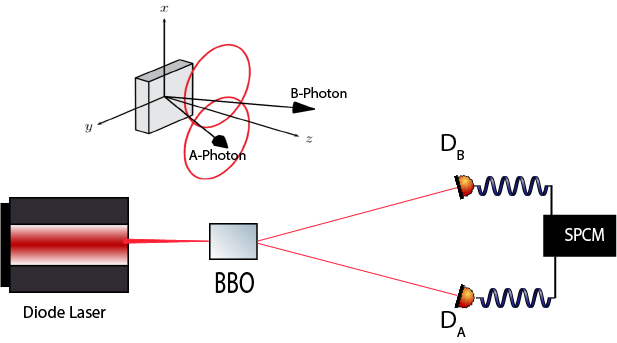
\includegraphics[width=0.65\textwidth]{Figures/spdcSimple.png}
 \caption{Simple Experimental setup for the type-II noncollinear SPDC process}
\label{fig:spdcSimple} 
\end{figure}


SPDC is an optical process in which a pump beam propagating in the $z$-direction is focused into a nonlinear crystal of length $L$. 
Depending on the polarisation direction of the produced photons, the nonlinear crystals 
can be classified in types. 
The type-0 crystal will produce pairs that are polarised in the source light direction. 
The type-I will produce pairs that are polarised in the perpendicular direction of the pump. 
The last type, type-II crystals will produce a pair of photons, 
one with the polarisation in the same direction as the pump, 
and the other one in the perpendicular direction. 
This procces can also be clasified according to the geometry, the relative direction from the crystal,
 in which the pair of down converted photons are going to be generated. The generated
 pair can emerge from the crystal in a collinear or non-collinear configuration. 
In Figure \ref{fig:spdcSimple} the non-collinear configuration is shown, where light is generated in two separated 
cones, for each polarisation, these light cones intercepts in two places, from where we will use pair the pair A-photon and B-photon.

For the rest of this monograph we will be focused in the type-II and non-collinear configuration. Using first order perturbation theory  and the paraxial approximation, the two-photon state
 coming out from the crystal, $\ket{\Psi}$, is given by \cite{omar}:
\begin{equation}
\begin{split}
\label{eq:stateFunComplex}
\ket{\Psi}=\int d\vec{q}_B d\vec{q}_A d\Omega_B d\Omega_A 
\times [\Phi(\vec{q}_B,\Omega_B;\vec{q}_A,\Omega_A) \hat{a}^{\dagger} (\Omega_B,\vec{q}_B) \hat{a}^{\dagger}(\Omega_A,\vec{q}_A) \\
+ \Phi(\vec{q}_A,\Omega_A;\vec{q}_B,\Omega_B) \hat{a}^{\dagger}(\Omega_B,\vec{q}_B) \hat{a}^{\dagger}(\Omega_A,\vec{q}_A)]   \ket{0}.  
\end{split}
\end{equation}
Where this state function depends on the transverse wave vectors $\vec{q}_n=(q_n^x,q_n^y)$ and frequency detuning, $\Omega_n=\omega_n-\omega_0^n$, 
around the central frequencies, $\omega_0^n$, for the photon at the path $A$ or $B$ ($n=A,B$).
The $\Phi(\vec{q}_B,\Omega_B;\vec{q}_A,\Omega_A)$ and $\Phi(\vec{q}_A,\Omega_A;\vec{q}_B,\Omega_B)$
are the mode functions or biphotons that contains all the information about the correlations
between the pair of down-converted photons. The operator $\hat{a}^{\dagger}$ indicates the creations of an $n$-polarized photon with transverse momentum $\vec{q}_n$, 
and frequency detuning $\Omega_n$. \\

For the light source that we will use in this monograph it is enough just one of the biphotons of the Eq. \ref{eq:stateFunComplex}. 
As will be shown later, this corresponds to put a pair of polarisers before the detection of the light (Sec. \ref{sec:pola})
. The Two-photon state reduces to:
\begin{equation}
\label{eq:stateFun}
\ket{\Psi}=\int d\vec{q}_B d\vec{q}_A d\Omega_B d\Omega_A 
\times [\Phi(\vec{q}_B,\Omega_B;\vec{q}_A,\Omega_A) \hat{a}^{\dagger} (\Omega_B,\vec{q}_B) \hat{a}^{\dagger}(\Omega_A,\vec{q}_A) 
] \ket{0}.  
\end{equation}

The mode function  $\Phi(\vec{q}_B,\Omega_B;\vec{q}_A,\Omega_A)$ is related with the joint probability of detecting both an $B$-polarized
photon, with tranverse momentum $\vec{q}_B$ and frequency detuning $\Omega_B$, at the detector $B$ 
and an $A$-polarized
photon, with tranverse momentum $\vec{q}_A$ and frequency detuning $\Omega_A$, at the detector $A$. 

\subsubsection{Phase matching conditions}
In particular, $\Phi(\vec{q}_B,\Omega_B;\vec{q}_A,\Omega_A)$ reads \cite{omar}:
\begin{equation}
\label{eq:mode}
\Phi(\vec{q}_B,\Omega_B;\vec{q}_A,\Omega_A) = \mathcal{N} \alpha(\Delta_0,\Delta_1) \beta(\Omega_B,\Omega_A) \times
sinc \left( \frac{\Delta_k L}{2} \right) e^{i \frac{\Delta_k L}{2}}.
\end{equation}
Where $\mathcal{N}$ is a normalisation constant, $\alpha(\Delta_0,\Delta_1)$
and $\beta(\Omega_B,\Omega_A)$yields the informations of the pump's transverse 
and spectral distribution, respectively, L is the length of the nonlinear crystal.
For the process that is happening inside the crystal, there are some conditions that have to be fulfilled. These conditions are related with the energy and momentum conservations inside the parametric down conversion process.
The terms $\Delta_0$, $\Delta_1$ and $\Delta_k$ are functions that result from the phase matching conditions and read:
\begin{equation}
\Delta_0=q_B^x + q_A^x.
\end{equation}
\begin{equation}
\Delta_1= q_A^y cos\phi_A + q_B^y cos\phi_B - N_B \Omega_B sin\phi_B + N_A \Omega_A sin\phi_A - \rho_B q_B^x sin\phi_B .
\end{equation}
\begin{equation}
\begin{split}
\Delta_k=N_p(\Omega_B+\Omega_A)-N_B\Omega_B cos\phi_B - N_A\Omega_A cos\phi_A \\ -q_B^y sin\Omega_B + q_A^y sin\Omega_A + \rho_p \Delta_0 - \rho_B q_B^x cos\phi_B.
\end{split}
\end{equation}
The angles $\phi_B$ and $\phi_A$ are the creation angles of the down-
converted photons with respect to the pump’s
propagation direction, whereas $\rho_p$ and $\rho_B$ are angles, they account for
the walk-off of the pump $p$ and the $B$ down-
converted photon, respectively.  $N_n=\frac{\delta k}{\delta \omega}$ denotes the inverse of the group velocity for each photon,
the change of the angular frequency $\omega$ against the angular wavenumber $k$.




\subsection{Spatial Correlations}\label{sec:spatialCorrelations}

In order to observe the correlations presented in \ref{eq:mode} we have to take into account some considerations about the descrption of the elements we have in the optical table.
First of all we have a pump beam with a Gaussian profile with waist $w_p$ 
in such way that $\alpha (\Delta_0,\Delta_1 ) \propto \text{exp}[-w_p^2 (\Delta_0^2 + \Delta_1^2 )/4]$, a CW pump laser, mathematically represented by
$\beta (\Omega_B , \Omega_A) \propto \delta(\Omega_B + \Omega_A)$. Making the aproximations for the sinc function by a Gaussian fuctions with the same width at $1/e^2$ of its maximum,
i.e., $sinc(x) \approx \text{exp}(-\gamma x^2)$ with $\gamma$ equal $0.193$.
The mode function reduces to:

\begin{equation}\label{eq:modeSim}
\begin{split}
\Phi(\vec{q}_B,\Omega_B;\vec{q}_A,\Omega_A) = \mathcal{N} \beta (\Omega_B , \Omega_A)
\times \\ \textit{exp}\left[ -\frac{w_p^2 (\Delta_0^2 + \Delta_1^2 )}{4}-\gamma \left(\frac{\Delta_k L}{2} \right)^2 + i\frac{\Delta_k L}{2} \right]  .
\end{split}
\end{equation}

As said before, we are interested in the spatial correlation that the photons 
exhibit. For these reason the frequency information has to be traced 
out. This is achieved by placing some interferometer filters before detection.
This spectral filters are modeled as $f_n (\Omega_n)=\text{exp}[-\Omega_n^2/(
4\sigma_n^2)]$, with bandwidth $\sigma_n$ chosen to achive a regimen where the 
spatial-spectral correlations are completely broken \cite{broke}. 
To achieve this mathematically we have to integrate \ref{eq:modeSim} around the
time variables:
\begin{equation}
\label{eq:modeSpa}
\tilde{\Phi}(\vec{q}_B,\vec{q}_A) = \int d\Omega_B d\Omega_A f_B(\Omega_B)f_A(\Omega_A) \Phi(\vec{q}_B,\Omega_B;\vec{q}_A,\Omega_A).
\end{equation}



The Biphoton then takes a quadratic form\cite{omar}:
\begin{equation}
\label{eq:quadratic}
\tilde{\Phi}(\vec{q}_B,\vec{q}_A)=N \textit{exp}\left[ -\frac{1}{2}x^T A x + i b^T x \right].
\end{equation}
where N is a normalization constant, that satisfies $\int \int | \tilde{\Phi}(\vec{q}_B,\vec{q}_A)|^2 d^2 \vec{q}_B d^2 \vec{q}_A = 1$. 
$x$ is a 4-dimensional vector defined as $x = (q^x_B, q^y_B ,q^x_A,q^y_A )$, $A$ 
is a 4 x 4 real-valued, symmetric, positive definite matrix and b is a 4-dimensional vector. 
A and b are defined from the phase-matching conditions of the SPDC process. $x^T$ and $b^T$ denote
 the transpose of $x$ and $b$. $A$ and $b$ are functions that depend of all the relevant 
parameters in the experiment such as the length of the crystal L, pump waist $w_p$, creation 
angles inside the crystal $\varphi_n$ and the width of the spectral filter $\sigma_n$.



\begin{figure}[h!]
\centering
{  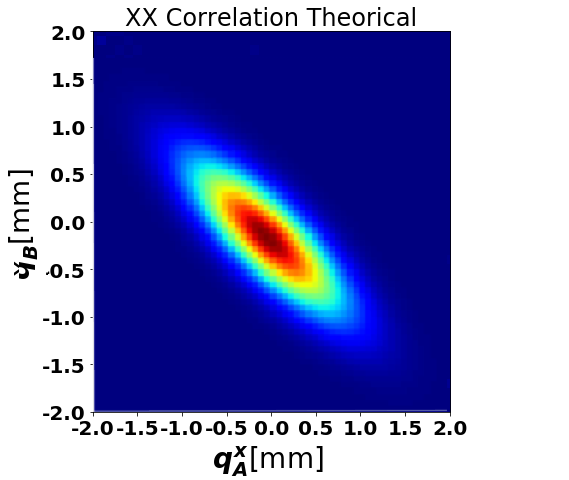
\includegraphics[width=0.48\textwidth]{Figures/theoricalxx.png} }
{  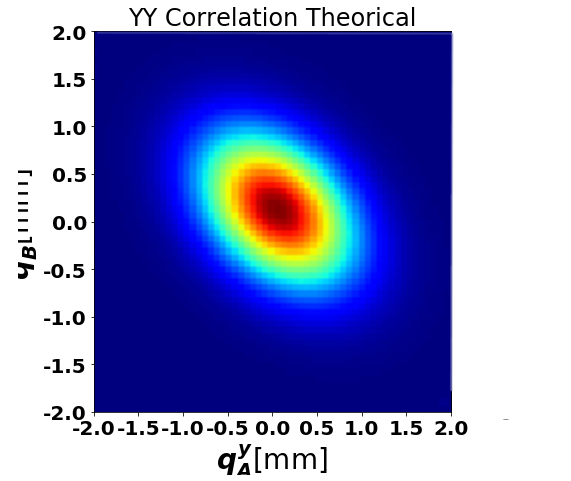
\includegraphics[width=0.48\textwidth]{Figures/theoricalyy.png} }
\caption{Theoretical Spatial correlations between a pair of down-converted photons, $w_p=91\mu m$}
 \label{fig:correThe}
\end{figure}
Figure \ref{fig:correThe} shows a pair of examples of how these correlations we are discussing about look like. These correlations have elliptical shape,
and show how strong is the posibility of detecting a photon at a given momentum. For example, looking 
at XX Correlation, there is a great chance
of detecting simultaneously a photon at $q^x_B=0$ and at $q^x_A=0$. Now if we keep looking at this XX correlation, we can also 
observe that detecting a photon at $q^x_B=0.5$, would constrain the posibles values of $q^x_A$ to values close to $-0.5$. This change in the sign
is an evidence of an anticorrelation between the photons in the XX direction. In Figure \ref{fig:correThe} we can also find the theoretical YY correlation. For this case we have a less narrower elipsis, meaning 
we have a less strong correlation in the YY direction. If we detect a photon at $q^y_B=0.5$, we would probably get 
another photon in the path A between $[-0.5,0.5]$ with almost equal probability for this range. It is clear that the more this correlations 
look like a circle, the correlation is less stronger . In contrast between more narrower the elipsis is, the stronger the correlation is. 
Another important fact from this analisys is that the direction of the elipsis give us a sense of the sign of the correlation, a negative correlation
is called an anticorrelation.



It is easy to think how a strong correlation should look like, a strong correlations in spatial variables would mean that if we have the position of one photon at the position 
$\vec{q}_B$ we immediately would know which $\vec{q}_A$ have the other photon, this king of ideal spatial correlation would look like a straigth line
really thin. Figure \ref{fig:idealCorre} shows this ideal correlation that  would be like having a relation of $\delta (\vec{q}_b -\vec{q}_a)$. 


\begin{figure}[h!]
\centering
{  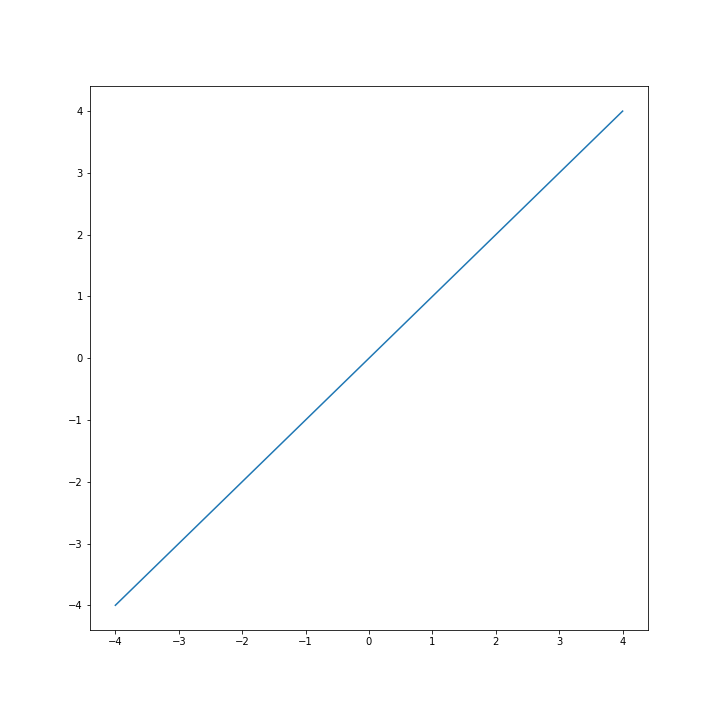
\includegraphics[width=0.48\textwidth]{Figures/idealPositiveCorrelation.png} }
{  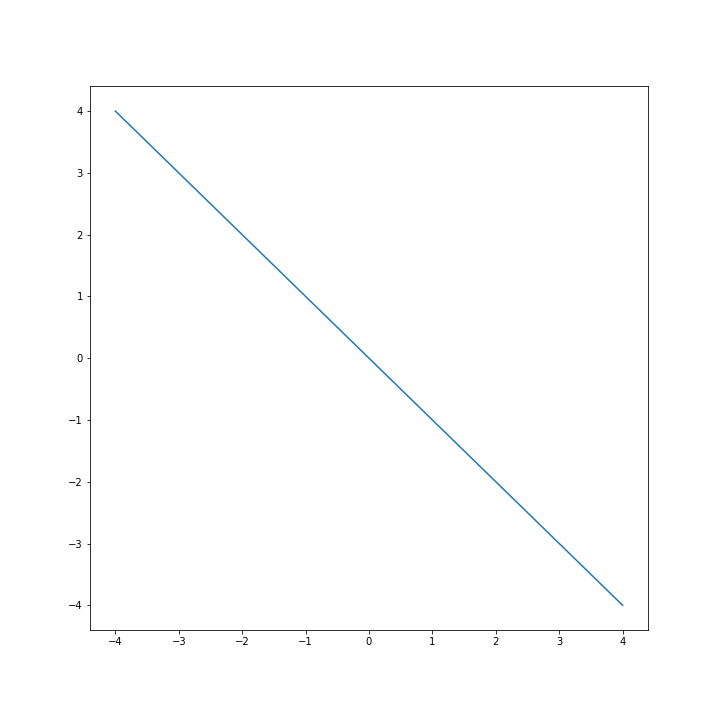
\includegraphics[width=0.48\textwidth]{Figures/idealNegativeCorrelation.png} }
\caption{Positive and Negative ideal spatial correlations}
 \label{fig:idealCorre}
\end{figure}

In the frame of this discussion, it would be useful to define a way to quantify the degree of spatial correlation.
We shall define a 'correlation parameter':

\begin{equation}
K^\lambda = \frac{C^\lambda_{si}}{\sqrt{C^\lambda_{ss}C^\lambda_{ii}}},
\end{equation}
calculated for each direction $(\lambda = x, y)$ from the covariance matrix $C^\lambda$ with elements $C^\lambda_{kj} = \langle q^\lambda_k q^\lambda_j \rangle - \langle q^\lambda_k \rangle \langle q^\lambda_j \rangle $.
This 'correlations parameter' is a measure of the linear correlation between two variables, in this case $q^{\lambda}_A$ and $q^{\lambda}_B$.

\begin{comment}

To have a general numerical approach to $\tilde{\Phi}(\vec{q_B},\vec{q_A})$, it is desired to 
writte it as generic correlations instead of the experimental parameters. This can be done by 
noticing that the amplitude of $\tilde{\Phi}(\vec{q_B},\vec{q_A})$ has the form of a 4-dimensional 
gaussian distribution, given by
\begin{equation}
f(x) = \tilde{N}e^{-\frac{1}{2}x^T \Sigma^{-1}x},
\label{Gaussian}
\end{equation}
where  $\tilde{N}$ is a normalization constant satisfying $\int f(x) d^4 x = 1$, $\Sigma^{-1}$ is 
the inverse of the covariance matrix that contains the correlations between the different elements
 of $x$. With $x_i$ {$i=0,1,2,3$}, $\Sigma$ can be written as:
\begin{equation}
\Sigma_{ij} = \sigma_{x_i} \sigma_{x_j} \rho_{x_i x_j}
\label{eq:Pearson}
\end{equation}
where $\sigma_i$ denotes de square root of the variance of  $x_i$ and $\rho_{x_i x_j}$ denotes the 
Pearson correlation coefficient between $x_i$ and $x_j$. This coefficient quantifies how strong is 
the linear correlation between $x_i$ and $x_j$\cite{shafer}.
By using Eq.(\ref{eq:Pearson}), the correlations between the spatial variables of the photons 
can be manually modified in Eq.(\ref{eq:quadratic}).

STILL WORK TO DO!!! \\

\end{comment}





\subsection{Tunable Spatial Correlation SPDC source light}
It is clear that both \ref{eq:modeSim} and \ref{eq:modeSpa} depend on $w_p$, the pump waist. If we change this 
parameter and keep the rest of the parameters constant, the term in the exponential function $[-w_p^2 (\Delta_0^2 + \Delta_1^2 )/4]$ will variate,
making changes in the shape of the original mode function. As it was mentioned here before and in \cite{omar}, the mode function
contains all the informations about the correlations of the generated down converted photons. Hence changing the pump waist $w_p$
will change the correlations of the generated pair of photons. In Figure \ref{fig:simCorrelations} is shown a new pair of correlations, but this
ones correspond to a different pump waist $w_p$. We can see the diferences with the ones presented in Fig. \ref{fig:correThe}, in this case we
have a positive correlation in the YY direction, meaning that we won't have a change of sing for $q^y$. Also, for this case, we have a stronger
correlation in the YY direction and we still have a anticorrelation in the XX direction, but this time is a weaker correlation.

\begin{figure}[h!]
\centering
{  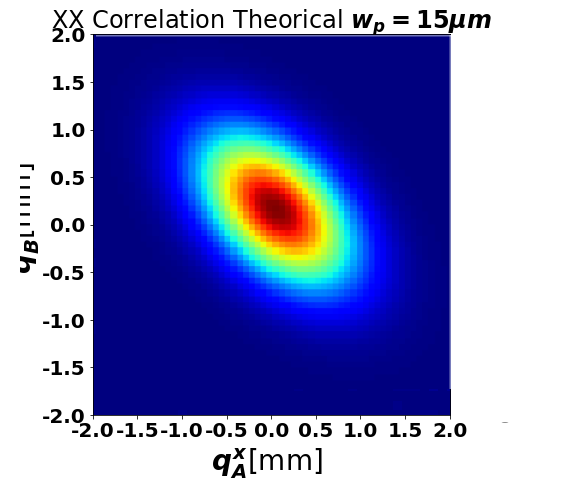
\includegraphics[width=0.48\textwidth]{Figures/correlationsWaistxx15.png} }
{  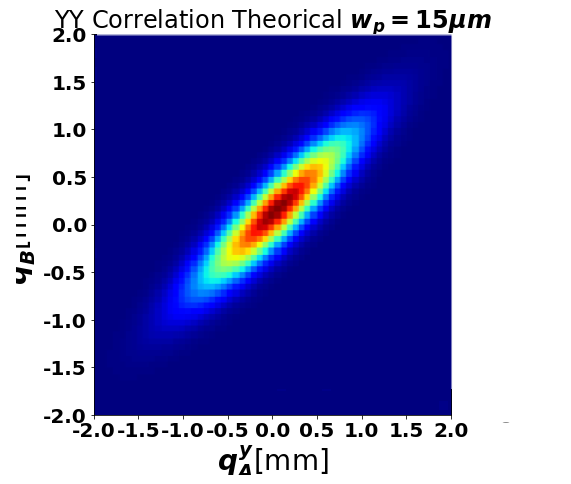
\includegraphics[width=0.48\textwidth]{Figures/correlationsWaistyy15.png} }
\caption{Simulated correlations $w_p=15\mu m$ }
 \label{fig:simCorrelations}
\end{figure}


\section{Imaging}
  
As said in the introduction, imaging is a process in which we make a reconstruction 
of an object using the spatial information of the light that were reflected, or scattered
from that object. This representation of the object can not be an exact copy. For example, when we forget
our glases, we see our surroundings blurred. The diference between 
having or not our glasses is that they will bost up our spatial resolution of the objects.



\subsection{Standard Imaging}


The concept of optical imaging was well developed in classical optics and the Figure
\ref{fig:imaging} schematically illustrates a standar imaging setup. In this setup 
an object is illuminated, an imaging lens is used 
to focus the scattered and reflected light from the object onto an image plane 
which is defined by the “Gaussian thin lens equation”\cite{hecht}:
\begin{equation}
\frac{1}{S_o}+\frac{1}{S_i}=\frac{1}{f},
\end{equation}
 where $S_o$ is the distance between the object and the imaging lens, $S_i$ the distance 
between the imaging lens and the image plane, and $f$ the focal lenght of the imaging lens. This equation defines
a point-to-point relationship between the object plane and the image plane: any radiation starting from a point on the object will colapse at a certain point at the image plane.
\\
\begin{figure}[h!]
\centering
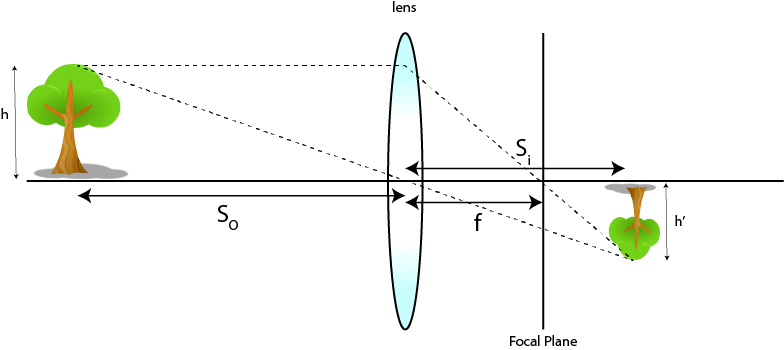
\includegraphics[width=0.6\textwidth]{Figures/imaging.png}
\caption{Optical imaging: a lens produces an image on an object at $S_i$. This distance is defined
by the Gaussian thin-lens equation} 
\label{fig:imaging}
\end{figure}
This one-to-one correspondence in the image-forming relationship between the object and the image planes produces a perfect image.
The observed image can be magnified or demagnified, for example, in the 
Figure \ref{fig:imaging} the original object is a tree, and it is demagnified at the image plane. This depends on which optical 
system are we using, what kind of lenses are involved and the distance between object and lenses.



The observed image is a reproduction of the illuminated object, mathematically
corresponding to a convolution between the object distribution fuction $ |T(\vec{r_o})|^2$ (aperture function) 
and a $\delta$-function, which is present for the perfect
point-to-point correspondence \cite{introquantumoptics}:
\begin{equation}
\label{eq:intensity}
\langle I(\vec{r_i}) \rangle =\int_{obj} d\vec{r_o} |T(\vec{r_o})|^2 \delta(\vec{r_o}+\frac{\vec{r_i}}{m}),
\end{equation}
where $\langle I(\vec{r_i})\rangle $ is the mean intensity at the image plane, $\vec{r_o}$ and $\vec{r_i}$ are 2-D vectors of the
transverse coordinates, $\vec{r_n}= (x_n,y_n)$, in the object and image planes, respectively, and
$m=S_i/S_o$ is the image magnification factor.

In a more real situation, we are limited by the finite size of the optical system, we may never obtain a perfect image.
The oscillating photons that form the image have constructive-destructive interference, turning the point-to-point correspondence into 
 a point-to-"spot" relationship. The $\delta$-function in the convolution of equation \ref{eq:intensity}
will be replaced by a point-to-"spot" image-forming function, or a point-spread function,
\begin{equation}
\label{eq:realIntensity}
\langle I(\vec{r_i}) \rangle =\int_{obj} d\vec{r_o} |T(\vec{r_o})|^2 \text{somb}^2[\frac{\pi D}{\lambda S_o} | \vec{r_o}+\frac{\vec{r_i}}{m}|],
\end{equation}

where the sombrero-like point-spread function is defined as 
somb$(x) \equiv  2J_1(x)/x$, with $J_1(x)$ the first-order Bessel function, $D$ the diameter of the imaging lens and $\lambda$ the wavelength of the light used.
the finite size of the spot is defined by $J_1(x)$ and 
determined by the ratio $D / \lambda S_o$. In Figure \ref{fig:bessel} we can appreciate the behaviour of the sombrero-like function for different
constants. The constants are define as $C=\frac{\pi D}{\lambda S_o}$ where we have to note some things in order to understand 
this function. First of all $\lambda$ is the light that we are using for the imaging process, so in the frame of this discussion 
about standar imaging, the light that is going to be used, is the light that the human eye can see($\sim 390-700 nm$). Restricting the light that
is going to be used leave us with two parameters to change. If we asume we will stay at a fixed distance $S_o$, Figure \ref{fig:bessel} shows
us that a narrower point-spread function is achievable increasing the size of the lens.
 
   



\begin{figure}[h!]
\centering
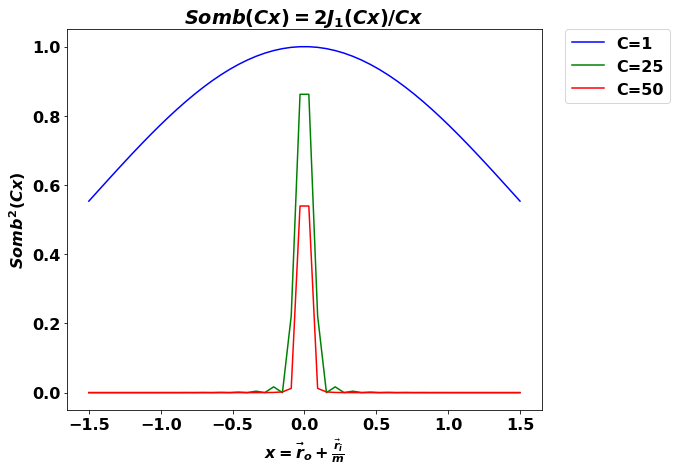
\includegraphics[width=0.6\textwidth]{Figures/bessel.png} 
\caption{sombrero-like function behaviour for differents constants }
\label{fig:bessel}
\end{figure}


 A narrower point-spread function turn into a high spatial resolution. Another daily situation in which we are forming images, is when we take a picture. Cameras manufacteres play 
with this functions to achieve a high spatial resolution, a spot-to-pixel correspondence.
For further informations about this "real life" situation check\cite{introquantumoptics} chapter 4 for further development.



\subsection{Two-photon Imaging}\label{twoPhotonImaging}

Two-photon imaging consist in reconstructing an image of an object. 
But in this case we use two dectector located in the two differents paths of the light. 
In Figure \ref{fig:twoPhotonSetup} we can appreciate a simple setup of the Two-photon technique.
We separate the light beam in two different paths, the photons traveling through the A path will reach
a $D_A$  point like detector, this detector have the ability to scan in the transverse direction.





\begin{figure}[h]
\centering
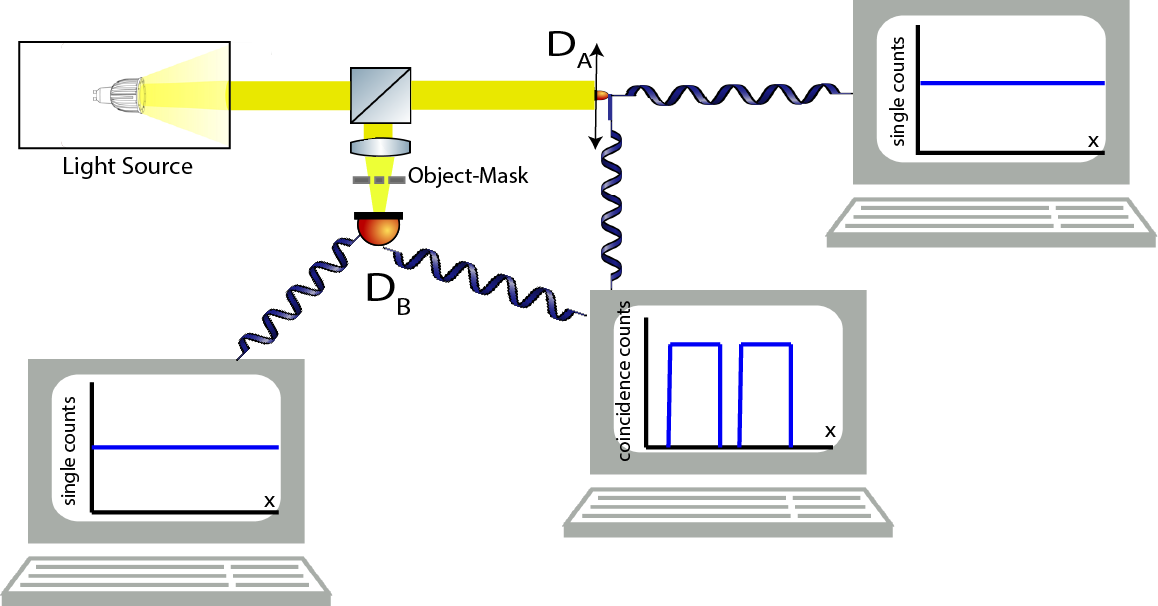
\includegraphics[width=0.75\textwidth]{Figures/twoPhotonSetupPC.png}
\caption{Simple schematic for the Two-photon Imaging. Only in the coincidence counts we can reconstruct the image} 
\label{fig:twoPhotonSetup}
\end{figure}

The light that were reflected in Figure \ref{fig:twoPhotonSetup} is denominated the B path.
This light goes through a imaging lens and then interacts with an object. After this, all light is collected
by a $D_B$ bucket detector, this detector loses all the spatial information about the light.
When we scan the $D_A$ detector in the transverse direction, we get a constant single 
counts, with no information what so ever about the object. When counting the photons that reached $D_B$
we also get a constant signal. 
However, if we go to the coincidence regime between $D_A$ and $D_B$, we are able to reconstruct the image.
This is done by counting every time we have a photon detected going througt the object $D_B$, and a photon at a certaint 
position $D_A(x_i)$ simultaneously. 



The standar imaging used the photons at the image plane to form the image. In other 
words it measures one photon per spot at the image plane. For the two-photon imaging, in certain 
aspects the behaviour is similar as that of the classical.
They both exhibit a similar point-to-point imaging-forming function, except the 
two-photon image is only reproducible in the joint-detection between two independent photodetectors,
and the point-to-point imaging-forming function is in the form of second-order correlation,
\begin{equation}\label{eq:coincidences}
R_{BA}(\vec{r_A})=\int_{obj} d\vec{r_B} |T(\vec{r_B})|^2 G^{(2)}(\vec{r_B},\vec{r_A}),
\end{equation}
where $R_{BA}(\vec{r_B})$ is the joint-detection counting rate between photodetectors $D_B$ and $D_A$.
$G^{(2)}(\vec{r_B},\vec{r_A})$ is a second-order correlation
function, corresponding to the probability of observing a joint photo-detection event
at the coordinates $\vec{r_B}$ and $\vec{r_A}$. The physics behing $G^{(2)}(\vec{r_B},\vec{r_A})$
is what changes between the light source used.

This second-order correlation functions is defined as\cite{introquantumoptics}:
\begin{equation}
G^{(2)} (\vec{r_B},\vec{r_A})= \frac{ \langle E^* (\vec{r_B}) E^* (\vec{r_A}) E^ (\vec{r_B}) E^ (\vec{r_A}) \rangle }{\langle |E^ (\vec{r_B})|^2 \rangle \langle |E^ (\vec{r_A})|^2 \rangle}.
\end{equation}
Where $E(\vec{r}_n)$ and $E^*(\vec{r}_n)$ are the electrical field and complex conjugate at the point $r_n$ with $n=A,B$. $E (\vec{r_n})|^2$ is defined by $E^*(\vec{r}_n) E(\vec{r}_n)$,
and $\langle ... \rangle$ stands for a statistical average.
%----------------------------------------------------------------------------------------
%	SECTION 1
%----------------------------------------------------------------------------------------
\subsubsection{LenslessTwo-photon Imaging using entangled photon}

In the previous section we introduced the notion of two-photon imaging , but we didn't care 
much about the nature of the light source. For this monograh we will use entangled photon as the 
light source. For now on we will focus on decribing the 
experimental setup presented in Figure \ref{fig:2f}. A diode laser is used to pump a BBO crystal, as a result of the
SPDC process, we obtain a pair of entangled photons in a noncollinear configuration. The down converted pairs travels
through a 2-f system. The A photon is then detected by $D_A$. In the path of the B photon, we place the object and then it is the $D_B$
bucket detector. It is important to note that in this setup there is no imaging lens, the used lenses are to define a very special plane at 
2f distance from the crystal, we will discus about it later in this section.


\begin{figure}[h]
\centering
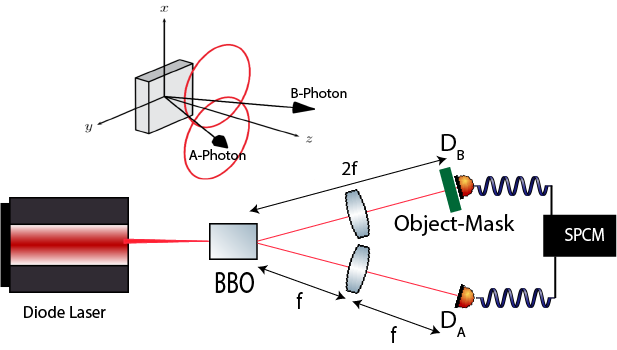
\includegraphics[width=0.75\textwidth]{Figures/simpleTwo.png}
\caption{Simple schematic for a Two-photon Imaging using entangled photons and a 2-f system} 
\label{fig:2f}
\end{figure}


\begin{comment}

The first two-photon imaging experiment was demonstrated by Pittman in 
1995\cite{pittman}. The schematic setup of the experiment is shown in the 
Figure \ref{fig:pittman}. \\ 

\begin{figure}[h]
\centering
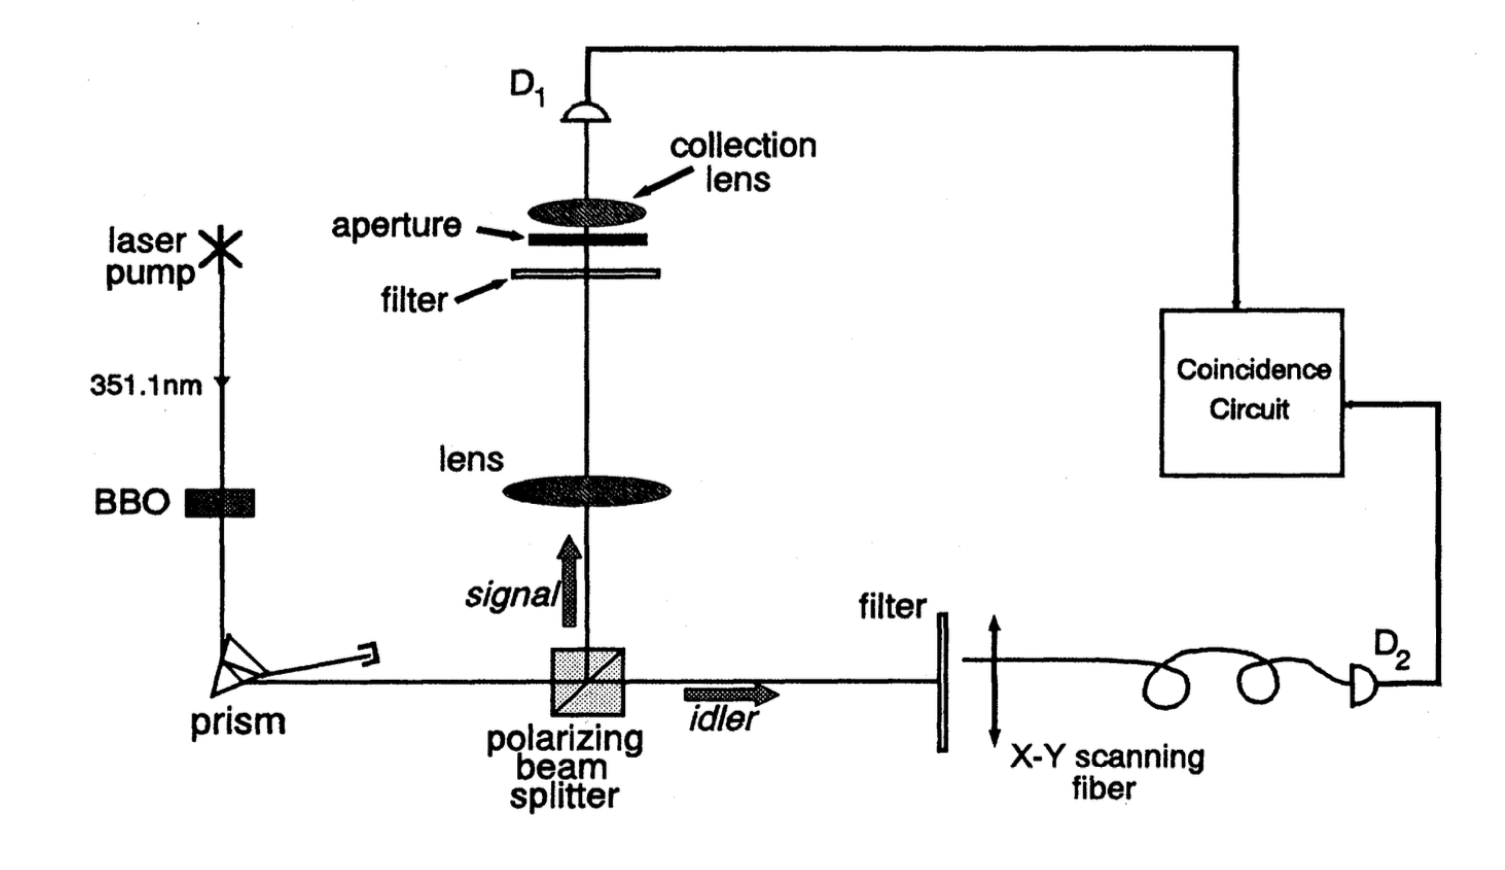
\includegraphics[width=0.75\textwidth]{Figures/pittman.png}
\caption{Schematic of the first "two-photon imaging" experimental setup, used by Pittman\cite{pittman}} 
\label{fig:pittman}
\end{figure}
 typo cristal, results




A continuous wave (CW) laser is used to pump a type-II nonlinear 
crystal to produce pairs of entangled photons. This pairs of orthogonally polarized signal and idler photons are the product
of the nonlinear optical process of spontaneous parametric down-conversion (SPDC).
The pair emerges from the crystal collinearly\footnote{The pairs emerge from the crystal nearly 
collinearly, with $\omega_s \simeq \omega_i \simeq \omega_p / 2$. where the subscript
letter stands for signal, idler and pump respectively}, it is separated by a dispersion prism, 
and then the signal and idler are sent in different directions by a polarization
beam slitting Glan-Thompson prism. 

The reflected signal beam passes through a 
convex lens with a $400mm$ focal length and illuminates an aperture\footnote{The aperture 
consisted of the letters UMBC, University of Maryland Baltimore County.}.
Before the aperture is placed a filter, 
this is a bandwidth spectral filters centered at the
wavelength $702.2 nm$. 
Behind the aperture is the detector package $D_1$. \\
%\begin{figure}[H]
%\centering
%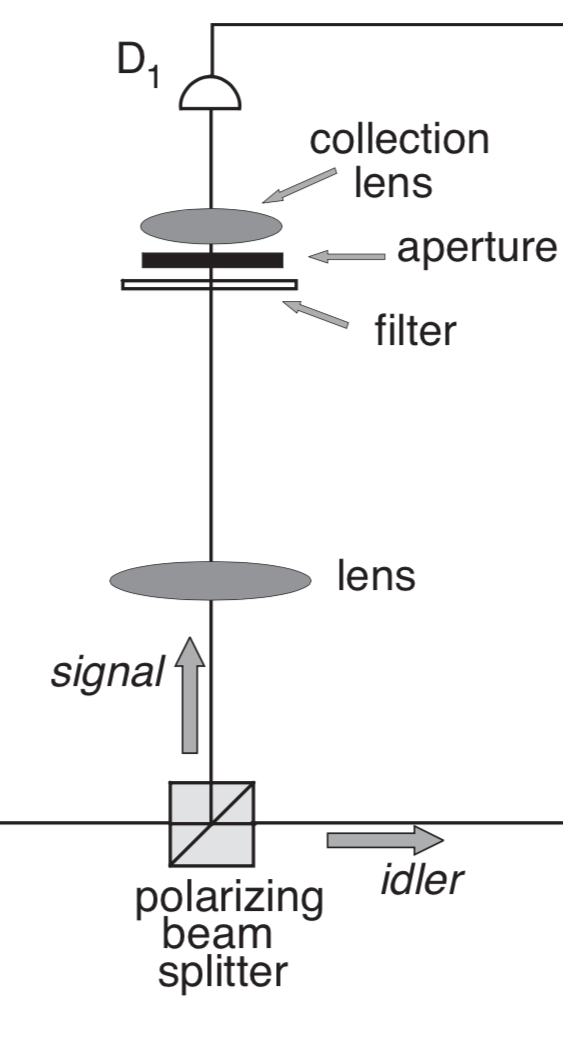
\includegraphics[width=0.24\textwidth]{Figures/signal.png}
%\caption{The reflected photon, called signal} 
%\label{fig:signal}
%\end{figure}


The transmitted idler beam is met by detector 
package $D_2$. The input tip of the fiber is scanned in the transverse 
plane. The counts are sent to a coincidence 
counting circuit with a $1.8ns$ acceptance window.
An important fact of this experiment is the use of a lens(collection lens) in the signal beam that establishes 
an image plane with the definitive point-by-point correspondence object(mask) plane.\\
\end{comment}




The main point of the section is to calculate Eq \ref{eq:coincidences} 
for this situation, we need to know 
the state of the biphoton at the output of the crystal, $\tilde{\Phi}_c(\vec{q}_c,\vec{q}_c)$ 


\begin{comment}
\begin{equation}
\label{eq:crystal}
\tilde{\Phi}_c(\vec{q}_c,\vec{q}_c)=N e^{\left[ -\frac{1}{2}x^T A x + i b^T x \right]}.
\end{equation}
\end{comment}


Then from this result we can use the fresnel propagation theory to analytically model the biphoton 
propagation in any arbitrary Two-photon Imaging/Lensless Two-photon Imaging setup.This propagation is done 
by determining the Green function of the optical path by which the beams will travel\cite{green}.



 
Since both path A and B have an identical 2-f system, we are at the called Fourier plane. It is 
well know that when the light goes through this system suffers a Fourier transform\cite{introquantumoptics}. It means that 
there is a relation beetwen
the initial $q_c$ initial transverse momentum at the crystal, and the $r_f$ final position of 
the photons. This relation is:



\begin{equation}\label{eq:fourier}
\vec{q}_{initial}=\frac{2 \pi}{\lambda f} \vec{r}_{final},
\end{equation}



where $\vec{q}_{initial}$ is the transverse momentum of the light before the 2-f system, $\vec{r}_{final}$ is the position of photon
after going through the lens and traveling a 2-f distance. $f$ stands for the focal length of the lenses used and $\lambda$ wavelength.\\
The Green function that propagates light with transverse momentum $\vec{q}$ from the source, to the
Fourier plane located at a position $\vec{r}_f$ is\cite{green}:
\begin{equation}\label{eq:green}
G(\vec{q},\vec{r}_f) = \int d^2 \vec{r}_l \int d^2 \vec{r}_c h(\vec{r}_f - \vec{r}_l,f) L_f(\vec{r}_l) h(\vec{r}_l - \vec{r}_c,f) e^{i q \cdot \vec{r}_c}.
\end{equation}
With $\vec{r}_c$ and $\vec{r}_l$ denoting the transverse position vectors in the plane of the crystal and the 
lens respectively. $h(\vec{r}_f - \vec{r}_l,f)$ and $h(\vec{r}_l - \vec{r}_c,f)$ are the Fresnel propagators\footnote{Fresnel Propagator: $h(\vec{r},z)=(- \frac{i}{\lambda z})e^{(i \frac{2 \pi z}{\lambda})} \Psi (\vec{r},z)$ 
with $\Psi(\vec{r},z) = e^{(i \frac{\pi}{\lambda z })\vec{r}^2}$. } that propagates light from $\vec{r}_l$ to $\vec{r}_f$ and 
$L_f (\vec{r})=\Psi(\vec{r},-f)$ is the thin-lens transfer function associated to a lens\cite{green}.
 \\
Taking advantage of the 2-f system as a Fourier transform to reduce the amount of calculations
, using the relation \ref{eq:fourier}, and after solving the integrals over $r_l$ and $r_c$, equation
 \ref{eq:green} can be written as:
\begin{equation}
\label{eq:greenSolve}
G(\vec{q},\vec{r}_f)=C e^{\frac{i \pi}{\lambda f} \vec{r}_f^2} e^{\frac{i \lambda f}{4 \pi} \vec{q}^2} \delta ( \vec{q} - \frac{2 \pi}{\lambda f}\vec{r}_f),
\end{equation}
where C is a complex constant.
Then we can finally propagate  the biphoton function
in terms of transverse momenta. Where $\Phi_1 (\vec{q}_B , \vec{q}_A )$ is the biphoton after traveling
through two arbitrary optical paths, it can be expressed
in terms of the corresponding Green functions and the
initial biphoton function, $\tilde{\Phi}_c(\vec{q}_c,\vec{q}_c)$, as:

\begin{equation}\label{eq:final}
\Phi_1 (\vec{q}_B , \vec{q}_A )= G_B(\vec{q}_B,\vec{r}_B) G_A(\vec{q}_A,\vec{r}_A) \tilde{\Phi}_c(\vec{q}_c,\vec{q}_c),
\end{equation}





where $\vec{r}_B$ and $\vec{r}_A$ denotes the photon position in the transverse plane at a 2-f distance from the 
crystal, the subscrip stand for the different path followed by light, Figure \ref{fig:2f}. The $G_B(\vec{q}_B,\vec{r}_B)$
and $G_A(\vec{q}_A,\vec{r}_A)$ are the green functions for each path, defined as in equation \ref{eq:greenSolve}, they are:
\begin{equation}\label{eq:B}
G_B(\vec{q}_B,\vec{r}_B)=G(\vec{q}_B,\vec{r}_B) \times T(\vec{r}_B) .
\end{equation}
\begin{equation}\label{eq:A}
G_A(\vec{q}_A,\vec{r}_A)=G(\vec{q}_A,\vec{r}_A).
\end{equation}
Where $T(\vec{r}_B)$ is the transfer function of the object, which is only present at the $B$ path, Figure \ref{fig:2f}.
Gathering all the previous results we can obtain $\Phi_1 (\vec{r}_B , \vec{r}_A )$. This is done by replacing
Eq. \ref{eq:B} and \ref{eq:A} into Eq. \ref{eq:final}, then evaluating the integrals over the transverse 
momentums, we obtain:
\begin{equation}\label{eq:finalBiphoton}
\Phi_1 (\vec{r}_B , \vec{r}_A )=C^2 T(\vec{r}_B) \Phi (\frac{2 \pi}{\lambda f}\vec{r}_B, \frac{2 \pi}{\lambda f}\vec{r}_A).
\end{equation}

This function describes the biphoton at the planes of the object and the scanning detector. It shows 
that the biphoton at the 2-f plane as a function of $\vec{r}_B$ and $\vec{r}_A$. If we take a closer look, this result
enable us to compute the biphoton at the 2-f plane by using Eq \ref{eq:quadratic} without the need to actually calculate its propagation, just by 
evaluating it with the Fourier relationship, \ref{eq:fourier}. This is specially usefull when we try to 
simulate this on a computer, the amount of calculations is significantly reduced by this fact.

As described at the beginning of this Section \ref{twoPhotonImaging}, we lose all the spatial information 
about the photon that interacts with the Object, B path, and this is done by placing a bucket detector that
gathers all light and send it to a multimode optic fiber, without saving any information about the position
of the photons in this path. From the mathematical point of view, the bucket detector is modeled
as: $\Phi_1 (\vec{r}_A) = C^2 \int d^2 \vec{r}_B T(\vec{r}_B) \Phi (\frac{2 \pi}{\lambda f}\vec{r}_B, \frac{2 \pi}{\lambda f}\vec{r}_A)$.
Using the fact that the coincidence counts that will be measured by the Detectors will be 
proportional to the magnitude square of the resulting biphoton function $\Phi_1 (\vec{r}_A)$\cite{introquantumoptics}.
\begin{equation}\label{eq:R}
R(\vec{r}_A) \propto  \int d^2 \vec{r}_B T(\vec{r}_B)^2 | \Phi (\frac{2 \pi}{\lambda f}\vec{r}_B, \frac{2 \pi}{\lambda f}\vec{r}_A) |^2
\end{equation}
Where $R(\vec{r}_A)$ is the function that describes de coincidences counts between de detectors $D_B$ and 
$D_A$ in Figure \ref{fig:2f}. $R(\vec{r}_A)$ is a function of the spatial positions, $(x_A,y_A)$
 of the detection plane at $D_A$. This function $R(\vec{r}_A)$ have the expected behaviour described
by $R_{BA}(\vec{r_A})$ in Eq. \ref{eq:coincidences}, where the second-order correlation function in this 
case is $\Phi (\frac{2 \pi}{\lambda f}\vec{r}_B, \frac{2 \pi}{\lambda f}\vec{r}_A)$, as we said, the function
containing all the informations about the correlations between the pair of down-converted photons. 
Moreover, Equation \ref{eq:R} indicates that the form of $\Phi(\vec{q}_B,\vec{q}_A)$ determines if $T(\vec{r}_B)$ can
be recovered in the coincidence count. Additionally, the type of spatial correlation in $\Phi(\vec{q}_B,\vec{q}_A)$
defines the orientation of the image obtained.

\subsubsection{Effect of the different spatial correlations}
If we want to observe the effect of differents spatial correlations in the obtained image, we need to take a look at Eq. \ref{eq:R}. This equation
describes me the obtained image as a function of the Biphoton. In here is where the spatial correlations are indicated, changing the spatial
correlations would mean to change the $\Phi (\frac{2 \pi}{\lambda f}\vec{r}_B, \frac{2 \pi}{\lambda f}\vec{r}_A)$. As said before, this experiment is a big project of the Quantum Optics group that was running way before
this monograph was started. This Eq \ref{eq:R} can be numerically solved, and this was done by one former group member. We can obtain numerically
the behaviour of $|\Phi (\frac{2 \pi}{\lambda f}\vec{r}_B, \frac{2 \pi}{\lambda f}\vec{r}_A)|^2$. 
In Figure \ref{fig:simTwo} there are two Two-photon images, each one of them corresponds to a different pump waist. The correlations for
$w_p=15 \mu m$ are in Figure \ref{fig:simCorrelations}, these correlations are related with the image we obtained. In the image for $w_p=15 \mu m$
we observe a wider elipsis for the $x$ values, while having a narrower part for the $y$ values. This is related to what was mentioned before,
for this waist, the YY correlations was stronger and positive, while for XX correlations we had a weaker anticorrelation. This anticorrelation
is observed in the change of position in the x direction.





\begin{figure}[h!]
\centering
{  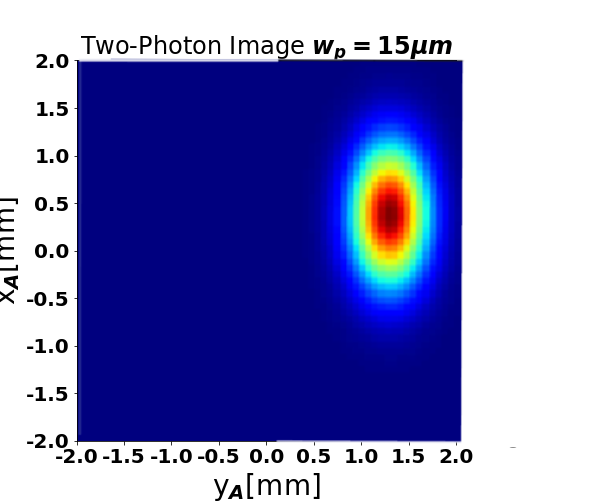
\includegraphics[width=0.48\textwidth]{Figures/twoPhoSq15.png} }
{  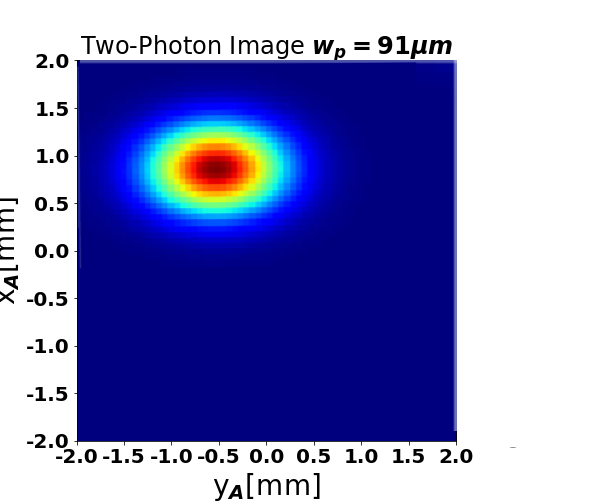
\includegraphics[width=0.48\textwidth]{Figures/twoPhoSq91.png} }
\caption{Simulated Two-photon images for two different waist, $w_p=15 \mu m$ and $w_p=91 \mu m$, Where $T(\vec{r}_B)$ is an square in the second quadrant.}
 \label{fig:simTwo}
\end{figure}




In the Figure \ref{fig:simTwo} we also find the Two-photon image for $w_p=91 \mu m$. The correlations for this waist are in Figure \ref{fig:correThe},
where we have a strong correlation in the XX direction and both of them are anticorrelations. The image change completely its original 
position in both direction, the photons present an anticorrelation. We had a weaker correlation in the YY direction, meaning loose spatial resolution in this direction.



